\documentclass[tikz,border=2pt]{standalone}

% Pure TikZ. pgfplots / fontspec / patterns.meta avoided so the compile
% works with a minimal TinyTeX install (see tikz_backend docstring).
\usetikzlibrary{arrows.meta, positioning, calc, patterns,
                decorations.pathmorphing}

% -- Colour palette (B&W-safe; every fill pairs with a pattern) --------
\definecolor{waterFill}{HTML}{e8eef5}
\definecolor{sandFill}{HTML}{e6ddc8}
\definecolor{scourFill}{HTML}{f2e8d8}
\definecolor{steelFill}{HTML}{1a1a1a}
\definecolor{accent}{HTML}{0b3d91}

% -- Geometry (1 cm = 100 mm model scale) ------------------------------
% Strongbox (inner dimensions):  1400 x 700 mm
%   Aluminium wall thickness drawn at 30 mm each side (exaggerated for
%   visual weight).
\def\boxW{14.0}     % strongbox inner width  (1400 mm)
\def\boxH{7.0}      % strongbox inner height (700  mm)
\def\wallT{0.3}     % wall thickness (30 mm, exaggerated)

% Soil bed: fills most of strongbox interior; free surface ~ 500 mm up.
\def\soilH{5.0}     % soil bed height inside strongbox (500 mm)
\def\waterTop{5.8}  % free water surface above soil surface (80 mm water)

% Foundation (centred on strongbox X, resting on sand bed surface).
\def\bucketR{0.57}  % bucket radius (D/2 = 57.1 mm model)
\def\bucketL{1.33}  % skirt length (132.9 mm model)
\def\tripodW{2.86}  % tripod base side L_base (286 mm)

% Tripod transition (drawn as triangular frame above the three buckets).
\def\tripodH{3.35}  % tripod height above mudline (335 mm, model)

% Tower stub (draw 2 cm then break)
\def\towerStubH{2.0}
\def\towerD{0.564}  % tower diameter 56.4 mm

% Scour hole (example, S/D = 0.58, the max tested)
\def\scourS{0.66}      % 0.58 * 114.3 mm = 66.3 mm model
\def\scourSlope{1.0}   % tan(45 deg) = 1
\def\scourOuterR{1.23} % D/2 + S at the surface

\begin{document}
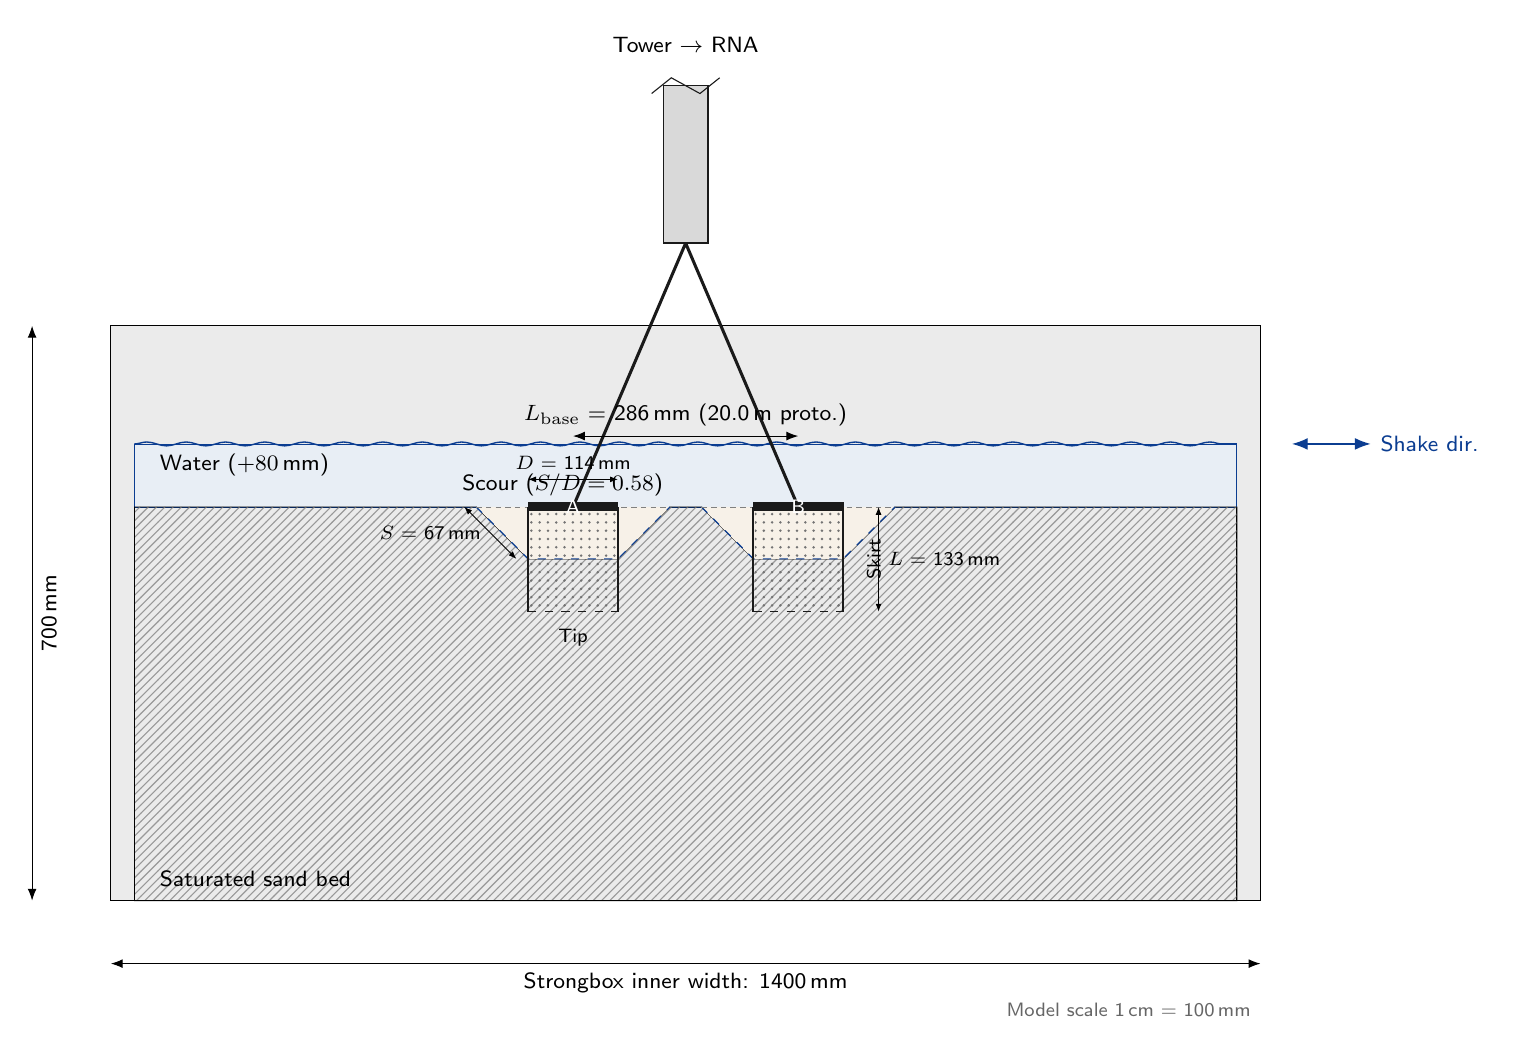
\begin{tikzpicture}[x=1cm, y=1cm, font=\sffamily\footnotesize]

    % ==========================================================
    % 1. NAMED COORDINATES
    % ==========================================================
    \coordinate (boxBL)   at (-\boxW/2 - \wallT, 0);
    \coordinate (boxBR)   at ( \boxW/2 + \wallT, 0);
    \coordinate (boxTL)   at (-\boxW/2 - \wallT, \boxH + \wallT);
    \coordinate (boxTR)   at ( \boxW/2 + \wallT, \boxH + \wallT);
    \coordinate (soilBL)  at (-\boxW/2, 0);
    \coordinate (soilBR)  at ( \boxW/2, 0);
    \coordinate (soilTL)  at (-\boxW/2, \soilH);
    \coordinate (soilTR)  at ( \boxW/2, \soilH);
    \coordinate (waterTL) at (-\boxW/2, \waterTop);
    \coordinate (waterTR) at ( \boxW/2, \waterTop);

    % Bucket A (left, visible in section)
    \coordinate (aLidL)   at (-\tripodW/2 - \bucketR, \soilH);
    \coordinate (aLidR)   at (-\tripodW/2 + \bucketR, \soilH);
    \coordinate (aTipL)   at (-\tripodW/2 - \bucketR, \soilH - \bucketL);
    \coordinate (aTipR)   at (-\tripodW/2 + \bucketR, \soilH - \bucketL);
    \coordinate (aCenLid) at (-\tripodW/2, \soilH);

    % Bucket B (right, visible in section)
    \coordinate (bLidL)   at ( \tripodW/2 - \bucketR, \soilH);
    \coordinate (bLidR)   at ( \tripodW/2 + \bucketR, \soilH);
    \coordinate (bTipL)   at ( \tripodW/2 - \bucketR, \soilH - \bucketL);
    \coordinate (bTipR)   at ( \tripodW/2 + \bucketR, \soilH - \bucketL);
    \coordinate (bCenLid) at ( \tripodW/2, \soilH);

    % Tripod apex (where the tower meets the tripod frame)
    \coordinate (tripodApex) at (0, \soilH + \tripodH);

    % Tower centreline + top of drawn stub + break
    \coordinate (towerBot)   at (0, \soilH + \tripodH);
    \coordinate (towerTop)   at (0, \soilH + \tripodH + \towerStubH);

    % ==========================================================
    % 2. STRONGBOX WALLS (drawn first so the fills sit inside)
    % ==========================================================
    \filldraw[fill=black!8, draw=black, line width=0.4pt]
        (boxBL) -- (boxBR) -- (boxTR) -- (boxTL) -- cycle
        [insert path={
            -- (soilBL) -- (soilBR) -- (soilTR) -- (soilTL) --
        (soilBL) -- cycle}];

    % ==========================================================
    % 3. WATER LAYER (top of strongbox interior)
    % ==========================================================
    \filldraw[fill=waterFill, draw=accent, line width=0.3pt]
        (soilTL) -- (soilTR) -- (waterTR) -- (waterTL) -- cycle;
    \draw[accent, line width=0.5pt, decorate,
          decoration={snake, amplitude=0.7pt, segment length=5mm}]
        (waterTL) -- (waterTR);

    % ==========================================================
    % 4. SAND BED (with scour hole carved out around each bucket)
    % ==========================================================
    % Scour hole boundaries (at surface level) for A and B
    \coordinate (aScourOL) at (-\tripodW/2 - \scourOuterR, \soilH);
    \coordinate (aScourOR) at (-\tripodW/2 + \scourOuterR, \soilH);
    \coordinate (aScourBL) at (-\tripodW/2 - \bucketR, \soilH - \scourS);
    \coordinate (aScourBR) at (-\tripodW/2 + \bucketR, \soilH - \scourS);
    \coordinate (bScourOL) at ( \tripodW/2 - \scourOuterR, \soilH);
    \coordinate (bScourOR) at ( \tripodW/2 + \scourOuterR, \soilH);
    \coordinate (bScourBL) at ( \tripodW/2 - \bucketR, \soilH - \scourS);
    \coordinate (bScourBR) at ( \tripodW/2 + \bucketR, \soilH - \scourS);

    \filldraw[fill=sandFill, pattern=north east lines,
              pattern color=black!40, draw=black, line width=0.3pt]
        (soilBL) -- (soilBR) -- (soilTR)
        % Scour B (right)
        -- (bScourOR) -- (bScourBR) -- (bScourBL) -- (bScourOL)
        % Between B and A
        -- (aScourOR) -- (aScourBR) -- (aScourBL) -- (aScourOL)
        -- (soilTL) -- cycle;

    % Lighter-toned scour holes (no fill pattern; dashed outline)
    \filldraw[fill=scourFill!60, draw=accent, line width=0.4pt, dashed]
        (aScourOL) -- (aScourBL) -- (aScourBR) -- (aScourOR);
    \filldraw[fill=scourFill!60, draw=accent, line width=0.4pt, dashed]
        (bScourOL) -- (bScourBL) -- (bScourBR) -- (bScourOR);

    % Original-mudline faint reference
    \draw[black!50, line width=0.3pt, dash pattern=on 2pt off 1.5pt]
        (aScourOL) -- (aScourOR);
    \draw[black!50, line width=0.3pt, dash pattern=on 2pt off 1.5pt]
        (bScourOL) -- (bScourOR);

    % ==========================================================
    % 5. BUCKETS (skirt + lid + dotted soil plug)
    % ==========================================================
    \foreach \lid in {aLidL,bLidL} {%
        % (skirt walls drawn per bucket below)
    }
    % Bucket A
    \draw[steelFill, line width=0.8pt] (aLidL) -- (aTipL);
    \draw[steelFill, line width=0.8pt] (aLidR) -- (aTipR);
    \draw[steelFill, line width=0.4pt, dashed] (aTipL) -- (aTipR);
    \filldraw[fill=steelFill, draw=steelFill]
        ($(aLidL)+(0,-0.05)$) rectangle ($(aLidR)+(0,0.05)$);
    \filldraw[fill=sandFill!80, draw=none,
              pattern=dots, pattern color=black!55]
        ($(aLidL)+(0.02,-0.05)$) rectangle ($(aTipR)+(-0.02,+0.03)$);

    % Bucket B
    \draw[steelFill, line width=0.8pt] (bLidL) -- (bTipL);
    \draw[steelFill, line width=0.8pt] (bLidR) -- (bTipR);
    \draw[steelFill, line width=0.4pt, dashed] (bTipL) -- (bTipR);
    \filldraw[fill=steelFill, draw=steelFill]
        ($(bLidL)+(0,-0.05)$) rectangle ($(bLidR)+(0,0.05)$);
    \filldraw[fill=sandFill!80, draw=none,
              pattern=dots, pattern color=black!55]
        ($(bLidL)+(0.02,-0.05)$) rectangle ($(bTipR)+(-0.02,+0.03)$);

    % ==========================================================
    % 6. TRIPOD FRAME (two braces, section plane view)
    % ==========================================================
    \draw[steelFill, line width=1.1pt]
        (aCenLid) -- (tripodApex) -- (bCenLid);
    \filldraw[fill=steelFill, draw=steelFill]
        ($(tripodApex) + (-0.18, 0)$) rectangle
        ($(tripodApex) + ( 0.18, 0.25)$);

    % ==========================================================
    % 7. TOWER STUB + BREAK + RNA LABEL
    % ==========================================================
    \filldraw[fill=black!15, draw=steelFill, line width=0.5pt]
        ($(towerBot)+(-\towerD/2, 0)$) rectangle
        ($(towerTop)+( \towerD/2, 0)$);

    % Tower break (zigzag)
    \draw[steelFill, line width=0.4pt]
        ($(towerTop)+(-\towerD/2 - 0.15, -0.1)$)
        -- ($(towerTop)+(-\towerD/2 + 0.1, 0.1)$)
        -- ($(towerTop)+( \towerD/2 - 0.1, -0.1)$)
        -- ($(towerTop)+( \towerD/2 + 0.15, 0.1)$);

    \node[font=\sffamily\footnotesize, anchor=south]
        at ($(towerTop) + (0, 0.3)$) {Tower $\rightarrow$ RNA};

    % ==========================================================
    % 8. DIMENSION ARROWS + LABELS
    % ==========================================================
    % Strongbox width (below the box)
    \draw[{Latex[length=1.5mm]}-{Latex[length=1.5mm]}, line width=0.35pt]
        ($(boxBL) + (0, -0.8)$) -- ($(boxBR) + (0, -0.8)$)
        node[midway, below, font=\sffamily\footnotesize]
            {Strongbox inner width: 1400\,mm};

    % Strongbox height (on the left)
    \draw[{Latex[length=1.5mm]}-{Latex[length=1.5mm]}, line width=0.35pt]
        ($(boxBL) + (-1.0, 0)$) -- ($(boxTL) + (-1.0, 0)$)
        node[midway, left, font=\sffamily\footnotesize, rotate=90, anchor=north]
            {700\,mm};

    % L_base (distance between bucket A and bucket B centres, above tripod apex)
    \draw[{Latex[length=1.5mm]}-{Latex[length=1.5mm]}, line width=0.35pt]
        ($(aCenLid) + (0, 0.9)$) -- ($(bCenLid) + (0, 0.9)$)
        node[midway, above, font=\sffamily\footnotesize]
            {$L_{\mathrm{base}}$ = 286\,mm (20.0\,m proto.)};

    % D (bucket diameter, above A)
    \draw[{Latex[length=1.0mm]}-{Latex[length=1.0mm]}, line width=0.3pt]
        ($(aLidL) + (0, 0.35)$) -- ($(aLidR) + (0, 0.35)$)
        node[midway, above, font=\sffamily\scriptsize]
            {$D$ = 114\,mm};

    % L (bucket skirt length, on the right of B)
    \draw[{Latex[length=1.0mm]}-{Latex[length=1.0mm]}, line width=0.3pt]
        ($(bLidR) + (0.45, 0)$) -- ($(bTipR) + (0.45, 0)$)
        node[midway, right, font=\sffamily\scriptsize]
            {$L$ = 133\,mm};

    % S (scour depth, between bucket A and its outer scour rim, left)
    \draw[{Latex[length=1.0mm]}-{Latex[length=1.0mm]}, line width=0.3pt]
        ($(aScourOL) + (-0.15, 0)$) -- ($(aScourBL) + (-0.15, 0)$)
        node[midway, left, font=\sffamily\scriptsize]
            {$S$ = 67\,mm};

    % ==========================================================
    % 9. CALLOUT LABELS
    % ==========================================================
    \node[anchor=north west, font=\sffamily\footnotesize]
        at ($(waterTL) + (0.2, 0.0)$) {Water ($+80$\,mm)};
    \node[anchor=north west, font=\sffamily\footnotesize]
        at ($(soilBL) + (0.2, 0.5)$) {Saturated sand bed};
    \node[anchor=north west, font=\sffamily\footnotesize]
        at ($(aScourOL) + (-0.3, 0.55)$)
        {Scour ($S/D = 0.58$)};
    \node[anchor=north, font=\sffamily\scriptsize,
          rotate=90]
        at ($(bLidR)!0.5!(bTipR) + (0.18, 0)$) {Skirt};
    \node[anchor=north, font=\sffamily\scriptsize]
        at ($(aTipL)!0.5!(aTipR) + (0, -0.1)$) {Tip};
    \node[anchor=center, font=\sffamily\scriptsize, white]
        at ($(aLidL)!0.5!(aLidR) + (0, 0.0)$) {A};
    \node[anchor=center, font=\sffamily\scriptsize, white]
        at ($(bLidL)!0.5!(bLidR) + (0, 0.0)$) {B};

    % ==========================================================
    % 10. SECTION-PLANE / SHAKE-DIRECTION INDICATOR
    % ==========================================================
    \draw[{Latex[length=2mm]}-{Latex[length=2mm]}, line width=0.5pt,
          color=accent]
        ($(boxTR) + (0.4, -1.5)$) -- ++(1.0, 0)
        node[right, font=\sffamily\footnotesize, color=accent]
            {Shake dir.};

    % Scale text
    \node[anchor=south east, font=\sffamily\scriptsize, color=black!60]
        at ($(boxBR) + (0, -1.6)$)
        {Model scale 1\,cm = 100\,mm};

\end{tikzpicture}
\end{document}
